%!Tex root = bare_conf.tex

\documentclass[conference]{IEEEtran}
\usepackage{graphicx}
\usepackage{hyperref}
\usepackage[capitalize]{cleveref}

\newcommand{\md} {\textsc{MCTSdvc} }
\newcommand{\cpu} {\textsc{MCTScpu} }
\newcommand{\gpu} {\textsc{MCTSgpu} }

\ifCLASSINFOpdf
\else
\fi

% correct bad hyphenation here
\hyphenation{op-tical net-works semi-conduc-tor}


\begin{document}

\title{Implementing Da Vinci Code Playing Algorithm based on Monte Carlo Tree Search}

% affiliations
\author{
\IEEEauthorblockN{Sangwoo Ji}
\IEEEauthorblockA{Dept. of CSE,
POSTECH\\
Pohang, Republic of Korea\\
sangwooji@postech.ac.kr}
\and
\IEEEauthorblockN{Wonup Jung}
\IEEEauthorblockA{Dept. of CSE,
POSTECH\\
Pohang, Republic of Korea\\
wonup@postech.ac.kr}
\and
\IEEEauthorblockN{Youngjoo Ko}
\IEEEauthorblockA{Dept. of CSE,
POSTECH\\
Pohang, Republic of Korea\\
y0108009@postech.ac.kr}}

\maketitle


% As a general rule, do not put math, special symbols or citations
% in the abstract
\begin{abstract}
%
\end{abstract}

% no keywords



\IEEEpeerreviewmaketitle


\section{Introduction}
% no \IEEEPARstart

% Popularity of A.I
Artificial intelligence defeated human play in the game `Go'.
As the number of cases in go is considered much larger than the number of cases in chess or Korean chess, go is treated as the unsolvable game to artificial intelligence.
However, AlphaGo defeated Korean top go player Sedol Lee, and the next version of AlphaGo defeated top go player Ke Jie.
Interestingly, AlphaGo decided to put a stone to a strange location that most go players could not understand~\cite{wierd_alphago}.
Many players shocked about the play of the AlphaGo and tried to learn the new strategies.

% Importance of MCTS
Monte Carlo tree search (MCTS) is a decision making algorithm that is used to implement AlphaGo~\cite{silver2016mastering_alphago}.
MCTS requires large number of simulations, and we hypothesized that large number of simulations led AlphaGo to the strange location.
The larger number of simulations, the better performance MCTS shows.
However, go has time limit for each turn, the number of simulations for each turn must be the bottleneck.

% Success of MCTS. Parallelism
AlphaGo put large number of hardware to increase the number of simulations~\cite{silver2016mastering_alphago}.
The paper-version AlphaGo used 48 CPUs and 8 GPUs.
Those hardware computing unit computes each simulation cases in parallel, and NEEDTO WRITE!~!~
The main factor of defeating human is not only improvement of algorithm, but also improvement of hardware.


% Drawback of MCTS. Case study by Da Vinci Code
However specific case of the game algorithm can harm the parallelism of MCTS.

% Prove of drawbacks (overhead)
We evaluated \cpu and \gpu to figure out main factor of decreasing performance.

% Future plan. Future work. (Discussion)


Monte Carlo Tree Search (MCTS) is a decision making algorithm which has been used for implementing aritifial intelligence(AI) widly. Since MCTS is used for games which proceed on real time, it should make decision within a limied time. However, we have to repeat a number of simulated games for good performance of MCTS. If MCTS doesn't have enough simulated games, MCTS can make wrong decision. Therefore parallelism of MCTS not only make right decision, but also reduce the time.\\
The Da vinci code is the kinds of board game. This game guesses the tiles of opponent based on 

\hfill mds
 
\hfill August 26, 2015
\section{Background}

\subsection{Da Vinci Code}

\subsection{Monte Carlo Tree Search}

MCTS is 

\section{Motivation}


% 일반적으로, implementation은 algorithm 뒤에 오는 경우가 많음.
\section{Method}
We implemented two versions of MCTS for Da Vinci code. 
Firstly, we implemented the MCTS algorithm for Da vinci code (\cpu) that is running upon CPU environment.
We used OpenMP to parallelize the algorithm.
Secondly, we implemented the same algorithm that is running upon GPU environment (\gpu).
We used cuda to implement and parallelize the algorithm.
% Both versions are implemented in parallel. 
In the remaining of this section, we describes each version of algorithm in detail. 
As we modified the algorithm due to compuation overhead, we explain the algorithm design considerations compared to the vanilla version of MCTS.

\subsection{Simplified Algorithm Design}

\begin{figure}
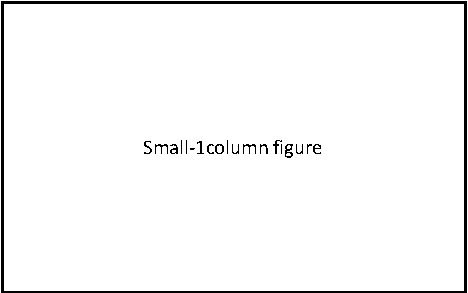
\includegraphics{figures/fit_1col.pdf}
\caption{FIX:Figure}
\label{fig:base_tree}
\end{figure}

 The \cref{fig:base_tree} shows the overall of MCTS for Da Vinci Code. 
 Each node has position and number which are values that a player guesses. Each depth means the game turn. 
 We implement simplified algorithm to reduce computation and proceed on real time, since original Da Vinci code has a lot of sibling nodes and child nodes which require a huge amount of computation and time limitation. 
 There are two case that we simplified. 
 First one is that a player who plays Da Vinci code has two behaviors in each turn, when he/she gussese the tiles. 
 Two behaviors are stop and keepping guess. 
 If the player guesses correctly, play can select stop or keepping guess. 
 Therefore, Original Da Vinci code makes depending on the player's choice. 
 However, we implemented Da Vinci code that only stop whether the player hits the tile or not. 
 Since original Da vinci code has numerous of child node which make the decision tree unbalanced, we decided to implemente simple Da Vinci code which only has stop behavior.
 
 Second one is original MCTS makes expansion to make decision make tree, but we simplified MCTS. Since Da Vinci Code has 000000 on each depth, the number of casese make a number of sibling nodes too hard to compute decision through MCTS. In addition, too many cases make wrong decision, because root node has nodes that have similar winning rate. Therefore, MCTS which we implemented has limitation of expansion. The \cref{fig:compare_expansion} shows the difference bewteen original MCTS and MCTS which we implemented. We make one expansion from root and then the remaining turns are proceeded randomly. The result of game updates expanded node from root and the MCTS doesn't make other expansion from frist depth. 


\subsection{Overall Implementation}
To make final MCTS both of CPU and GPU, each thread make small MCTS by simulating a couple of games.
At this time, MCTS is conducted based on current state of own player and an oppenent.
As playing some games within a thread, a simulation makes small MCTS.
Each game in a thread expands the child node from root. 
When the game expands the child node at the frist turn in a thread, the game proceed randomly. 
The result of game rolls out parent node and is updated on the node which is depth one. 
The next game also expands the child node from the root and update the result of game to expanded node (depth one).
Each tread repeats this routin to make small MCTS. 
The threads have small trees which is from simulation and these trees are combined to final MCTS which is used for decision making in Da Vinci code. 
The \cref{fig:implementation} shows the overall process how the MCTS is conducted.
When the player comes to the turn, threads make final MCTS based on current state of the player and the oppenent. 
The player makes the decision based on the final MCTS. 

\subsection{Implementation of MCTS based on CPU}
MCTS needs many simulated play repeatly to make good decision. 
Parallelism can make MCTS construct good decision tree in a short period due to computating simultaneously. 
MCTS based on CPU is implemented by openMP to utilize parallelism. Each thread computes some turns and derivates a result(win or lose). 
After finish derivation of result, all results from each thread are combined one MCTS.


\subsection{Implementation of MCTS based on GPU}
As we mentioned, MCTS need parallelism to computation many cases for good decision. 
In GPU version, we use CUDA for paraller computation. 
Each tread computes a couple of turns and derivates a result(win or lose) as same as CPU version. 
After finish derivation of result, the results from each tread are combined final MCTS. 


\section{Evaluation}
We implemented MCTS for Da Vincicode upon 4-CPU(Pascal Titan Xp) and 12-core CPU.
We measure the execution time to analysis the dominant factor of time consuming.
We evaluate the performance and difference between CPU based MCTS and GPU based MCTS to measure from the number of simulation per second.

\subsection{Execution Time}
We mesure the execution time by varying the number of simulations from 1 to $10^7$ and calculate average values on 5 times execution. 
The \cref{fig:time_consuming} shows the execution time which CPU measures using 12 threads and GPU measures using 32 threads
As increasing the number of simulations, the execution time also increases. Therefore, the number of simulation is dominant factor of time consuming. 

The \cref{fig:time_consuming} shows that the execution is not much different when the number of simulations is small. 
However, as the number of simulations increases, the number of simulations and the execution time are proportional.
The reason is when the number of simulation is small, the memory access to the large array becomes the key factor of the performance. However, when the number of simulation is large, the computing becomes the key factor. Therefore the performance (execution time) is proportional to the number of simulations.

\subsection{The Number of Simulation per Second}
\subsubsection{CPU}
The \cref{fig:cpu_num_simulation} shows the result of the number of simulation per second over increasing number of threads of CPU. As incresing threads, the number of simulations per second also increases linearly. 
However, you can see the number of simulations decrease if the number of threads exceeds 12. 
The reason why the number of simulations decrease is that we have only 12 core. In other word, the number of physical cores is the scalability bootleneck. 
Therefore, it can be seen that the performance increases linearly with the number of cores in the CPU. 
\subsubsection{GPU}
The \cref{fig:gpu_num_simulation} shows the result of the number of simulation per second over increasing number of threads of GPU. 
Unlike the \cref{fig:cpu_num_simulation}, the \cref{fig:gpu_num_simulation} shows the non-linear shape. 
In addition, the graph has instant performance degradation at the middle despite increasing the number of threads. 
This is because cache misses increase as the number of thread is used, and memory bottlenecks from cache misses are higher than computaion performance obtained by increasing threads in CPU as mentioned in [cite].

In MCTS based on GPU, the threads which are already finished should wait until the thread which has the most number of turns ends. 
Because other threads need to wait for the longest thread, the MCTS based on GPU should be the weak scaling which takes the same amount of time to increase the number of threads.
However, the \cref{fig:gpu_thread_time} which  shows that weak scaling is not sustained. 

% An example of a floating figure using the graphicx package.
% Note that \label must occur AFTER (or within) \caption.
% For figures, \caption should occur after the \includegraphics.
% Note that IEEEtran v1.7 and later has special internal code that
% is designed to preserve the operation of \label within \caption
% even when the captionsoff option is in effect. However, because
% of issues like this, it may be the safest practice to put all your
% \label just after \caption rather than within \caption{}.
%
% Reminder: the "draftcls" or "draftclsnofoot", not "draft", class
% option should be used if it is desired that the figures are to be
% displayed while in draft mode.
%
%\begin{figure}[!t]
%\centering
%\includegraphics[width=2.5in]{myfigure}
% where an .eps filename suffix will be assumed under latex, 
% and a .pdf suffix will be assumed for pdflatex; or what has been declared
% via \DeclareGraphicsExtensions.
%\caption{Simulation results for the network.}
%\label{fig_sim}
%\end{figure}

% Note that the IEEE typically puts floats only at the top, even when this
% results in a large percentage of a column being occupied by floats.


% An example of a double column floating figure using two subfigures.
% (The subfig.sty package must be loaded for this to work.)
% The subfigure \label commands are set within each subfloat command,
% and the \label for the overall figure must come after \caption.
% \hfil is used as a separator to get equal spacing.
% Watch out that the combined width of all the subfigures on a 
% line do not exceed the text width or a line break will occur.
%
%\begin{figure*}[!t]
%\centering
%\subfloat[Case I]{\includegraphics[width=2.5in]{box}%
%\label{fig_first_case}}
%\hfil
%\subfloat[Case II]{\includegraphics[width=2.5in]{box}%
%\label{fig_second_case}}
%\caption{Simulation results for the network.}
%\label{fig_sim}
%\end{figure*}
%
% Note that often IEEE papers with subfigures do not employ subfigure
% captions (using the optional argument to \subfloat[]), but instead will
% reference/describe all of them (a), (b), etc., within the main caption.
% Be aware that for subfig.sty to generate the (a), (b), etc., subfigure
% labels, the optional argument to \subfloat must be present. If a
% subcaption is not desired, just leave its contents blank,
% e.g., \subfloat[].


% An example of a floating table. Note that, for IEEE style tables, the
% \caption command should come BEFORE the table and, given that table
% captions serve much like titles, are usually capitalized except for words
% such as a, an, and, as, at, but, by, for, in, nor, of, on, or, the, to
% and up, which are usually not capitalized unless they are the first or
% last word of the caption. Table text will default to \footnotesize as
% the IEEE normally uses this smaller font for tables.
% The \label must come after \caption as always.
%
%\begin{table}[!t]
%% increase table row spacing, adjust to taste
%\renewcommand{\arraystretch}{1.3}
% if using array.sty, it might be a good idea to tweak the value of
% \extrarowheight as needed to properly center the text within the cells
%\caption{An Example of a Table}
%\label{table_example}
%\centering
%% Some packages, such as MDW tools, offer better commands for making tables
%% than the plain LaTeX2e tabular which is used here.
%\begin{tabular}{|c||c|}
%\hline
%One & Two\\
%\hline
%Three & Four\\
%\hline
%\end{tabular}
%\end{table}


% Note that the IEEE does not put floats in the very first column
% - or typically anywhere on the first page for that matter. Also,
% in-text middle ("here") positioning is typically not used, but it
% is allowed and encouraged for Computer Society conferences (but
% not Computer Society journals). Most IEEE journals/conferences use
% top floats exclusively. 
% Note that, LaTeX2e, unlike IEEE journals/conferences, places
% footnotes above bottom floats. This can be corrected via the
% \fnbelowfloat command of the stfloats package.




\section{Conclusion}
The conclusion goes here.




% conference papers do not normally have an appendix


% use section* for acknowledgment
\section*{Acknowledgment}


The authors would like to thank...





% trigger a \newpage just before the given reference
% number - used to balance the columns on the last page
% adjust value as needed - may need to be readjusted if
% the document is modified later
%\IEEEtriggeratref{8}
% The "triggered" command can be changed if desired:
%\IEEEtriggercmd{\enlargethispage{-5in}}

% references section

% can use a bibliography generated by BibTeX as a .bbl file
% BibTeX documentation can be easily obtained at:
% http://mirror.ctan.org/biblio/bibtex/contrib/doc/
% The IEEEtran BibTeX style support page is at:
% http://www.michaelshell.org/tex/ieeetran/bibtex/
%\bibliographystyle{IEEEtran}
% argument is your BibTeX string definitions and bibliography database(s)
%\bibliography{IEEEabrv,../bib/paper}
%
% <OR> manually copy in the resultant .bbl file
% set second argument of \begin to the number of references
% (used to reserve space for the reference number labels box)

% \begin{thebibliography}
\bibliographystyle{IEEEtran}
\bibliography{reference}
% \end{thebibliography}




% that's all folks
\end{document}


